\section{空基类优化(EBCO)}

C++类通常是“空的”,内部表示在运行时不需要内存位。对于包含类型成员、非虚函数成员和静态数据成员的类,通常是这样。另一方面,非静态数据成员、虚函数和虚基类在运行时确实需要一些内存。

即使是空类,其大小也是非零的。若想验证这一点,可以试试下面的代码:

\filename{inherit/empty.cpp}
\begin{cpp}
#include <iostream>

class EmptyClass {
};

int main()
{
	std::cout << "sizeof(EmptyClass): " << sizeof(EmptyClass) << ’\n’;
}
\end{cpp}

对于多数平台,这个程序将输出1作为EmptyClass的大小。一些系统对类类型有更严格的对齐要求,可能会打印另一个小整数(通常为4)。

\subsection{结构布置原则}

C++的设计者有各种理由来避免零大小的类。一个由零大小类组成的数组的大小应该也为零,但是指针算法的属性将不再适用。假设ZeroSizedT是一个零大小的类型:

\begin{cpp}
ZeroSizedT z[10];
...
&z[i] - &z[j] // compute distance between pointers/addresses
\end{cpp}

前一个示例中的差异是通过两个地址之间的字节数,除以它所指向的类型的大小得到的,但当该大小为零时,这显然不令人满意。

然而,即使在C++中没有零大小的类型,C++标准指定一个空类作为基类时,不需要为它分配空间,只要不分配到与另一个相同类型对象或子对象相同地址中即可。我们通过一些示例来阐明这个空基类优化(EBCO)在实践中的含义:

\filename{inherit/ebco1.cpp}
\begin{cpp}
#include <iostream>

class Empty {
	using Int = int; // type alias members don’t make a class nonempty
};

class EmptyToo : public Empty {
};

class EmptyThree : public EmptyToo {
};

int main()
{
	std::cout << "sizeof(Empty): " << sizeof(Empty) << ’\n’;
	std::cout << "sizeof(EmptyToo): " << sizeof(EmptyToo) << ’\n’;
	std::cout << "sizeof(EmptyThree): " << sizeof(EmptyThree) << ’\n’;
}
\end{cpp}

若编译器实现了EBCO,将为每个类打印相同的大小,但这些类的大小都不是0(参见图21.1)。类EmptyToo中,类Empty没有赋予空间,优化过的空基类(没有其他基类)的空类也是空的。这解释了,为什么类EmptyThree也可以具有与类Empty相同的大小。若编译器没有实现EBCO,将输出不同的大小(参见图21.2)。

\begin{center}
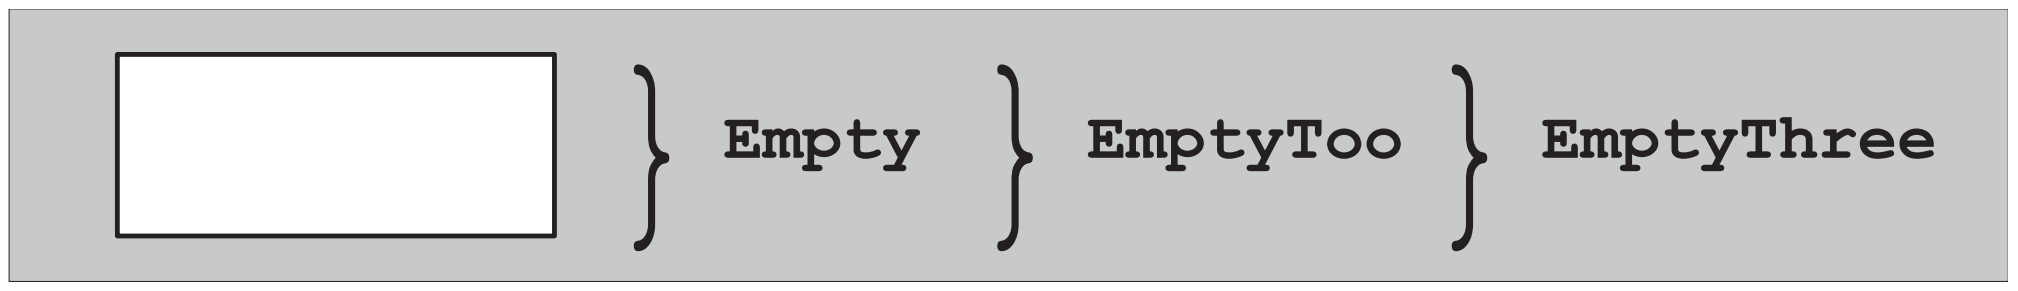
\includegraphics[width=0.8\textwidth]{part3/ch21/images/1.png} \\
图21.1. EmptyThree的结构,由实现EBCO的编译器
\end{center}

\begin{center}
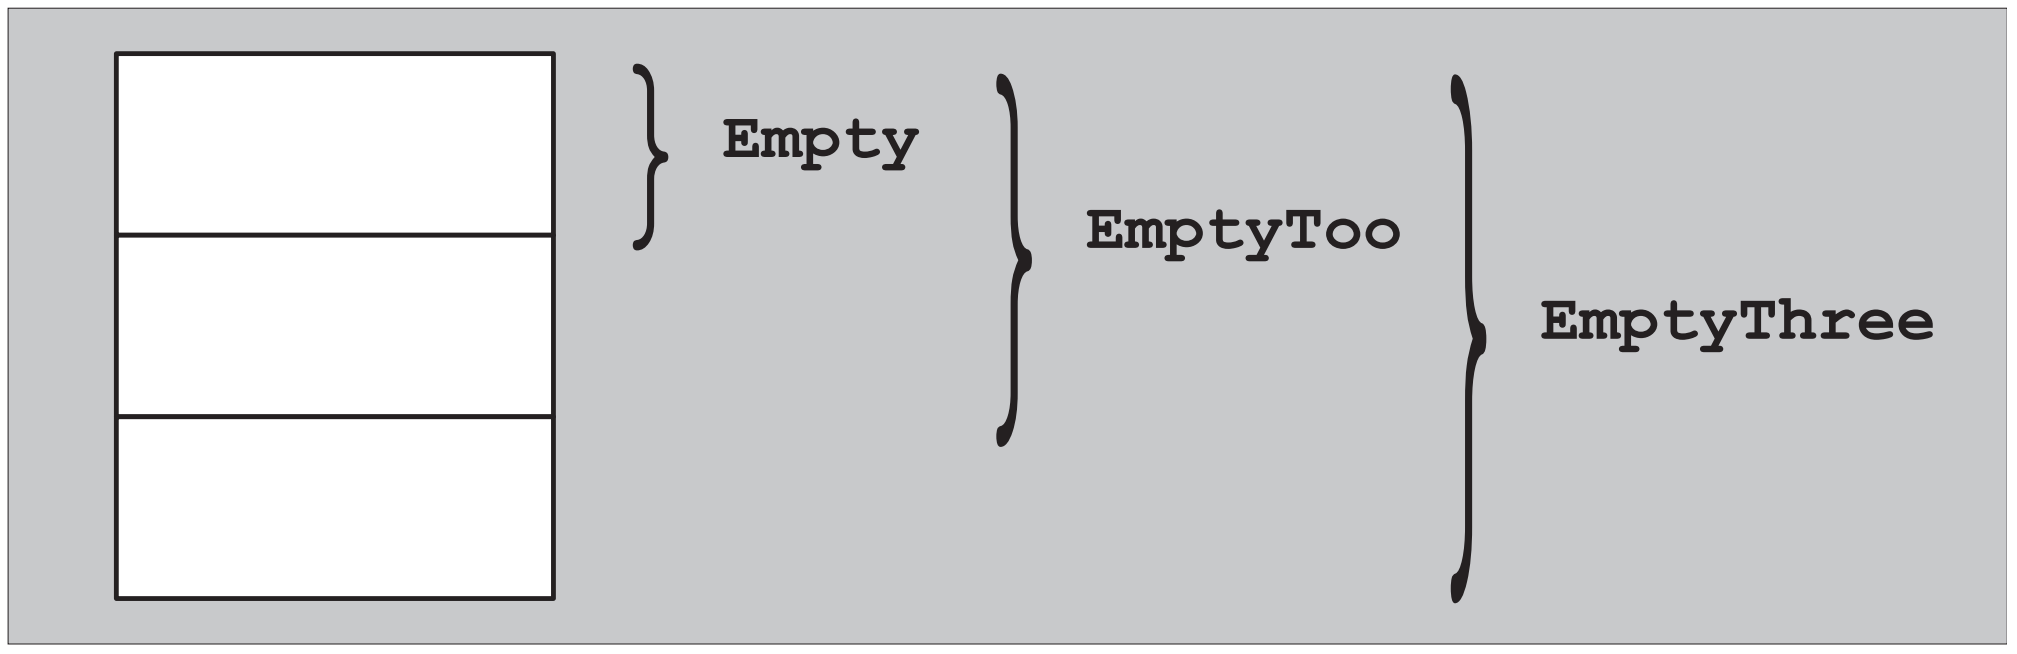
\includegraphics[width=0.8\textwidth]{part3/ch21/images/2.png} \\
图21.2. EmptyThree的结构,由未实现EBCO的编译器
\end{center}

考虑遇到EBCO约束的情况:

\filename{inherit/ebco2.cpp}
\begin{cpp}
#include <iostream>

class Empty {
	using Int = int; // type alias members don’t make a class nonempty
};

class EmptyToo : public Empty {
};

class NonEmpty : public Empty, public EmptyToo {
};

int main()
{
	std::cout << "sizeof(Empty): " << sizeof(Empty) << ’\n’;
	std::cout << "sizeof(EmptyToo): " << sizeof(EmptyToo) << ’\n’;
	std::cout << "sizeof(NonEmpty): " << sizeof(NonEmpty) << ’\n’;
}
\end{cpp}

NonEmpty类不是一个空类!没有任何成员,基类也没有。但NonEmpty的基类Empty和EmptyToo不能分配到相同地址,这将导致EmptyToo的基类Empty与NonEmpty的基类Empty位于相同的地址。相同类型的两个子对象将以相同的偏移量结束,而这是C++的对象布局规则不允许的。可以想象,Empty基子对象中的一个放置在偏移量“0字节”处,另一个放置在偏移量“1字节”处,但是完整的NonEmpty对象仍然不能有1字节的大小,因为在两个NonEmpty对象的数组中,所以第一个元素的Empty子对象不能与第二个元素的Empty子对象在同一地址(参见图21.3)。

\begin{center}
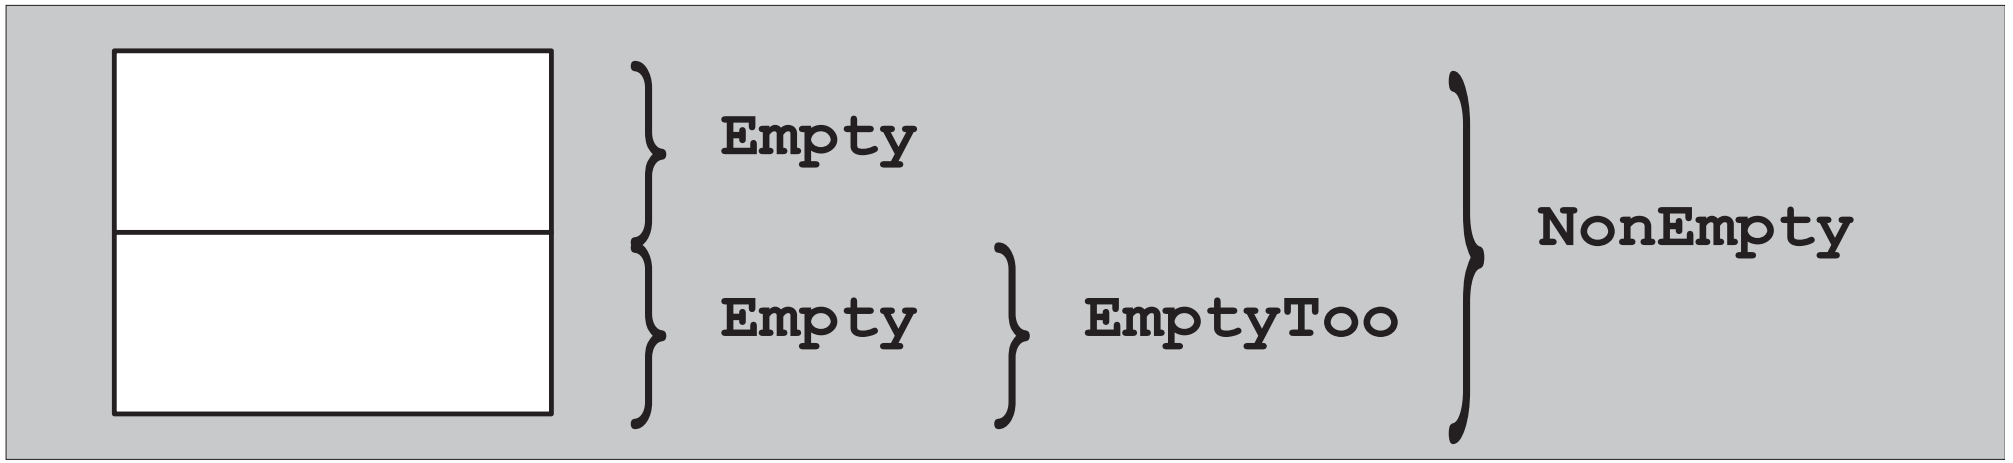
\includegraphics[width=0.8\textwidth]{part3/ch21/images/3.png} \\
图21.3. 实现EBCO的编译器的非空结构
\end{center}

对EBCO进行约束的基本原理源于这样一个事实,即能够比较两个指针是否指向同一个对象。指针在内部表示为地址,必须确保两个不同的地址(即指针值)对应两个不同的对象。

这个限制看起来可能不重要,但在实践中,经常会遇到这种情况,因为许多类倾向于使用一小组空类定义一些常见类型别名的空类继承。当此类中的两个子对象同时用于同一完整对象时,就抑制了优化。

即使有这个约束,EBCO仍然是模板库的重要优化,因为许多技术依赖于基类引入,只是为了引入新类型别名或提供额外的功能,而不添加新数据。

\subsection{基类的成员}

EBCO对于数据成员没有同等功能,因为(其他方面)会在成员指针的表示方面产生一些问题。因此,有时需要将成员变量实现为(私有)基类,这很有挑战性。

这个问题在模板上下文中最有趣,模板参数经常使用空类类型替换,但不能依赖于此规则。若对模板类型参数一无所知,就不能使用EBCO。考虑一下下面这个例子:

\begin{cpp}
template<typename T1, typename T2>
class MyClass {
	private:
	T1 a;
	T2 b;
	...
};
\end{cpp}

完全有可能使用空类类型替代一个或两个模板参数。若是这样,那么MyClass<T1,T2>的表示可能是次优的,并且可能为每个MyClass<T1,T2>的实例浪费一个字符的内存。

可以通过将模板参数设置为基类来避免这种情况发生:

\begin{cpp}
template<typename T1, typename T2>
class MyClass : private T1, private T2 {
};
\end{cpp}

这种简单的替代方法也存在一些问题:

\begin{itemize}
\item 
当使用非类类型或联合类型替代T1或T2时,这种方式无效。

\item 
当两个参数替换为相同类型时,也不起作用(可以通过添加另一层继承来解决)。

\item 
类可以是final类,在这种情况下,试图对它进行继承将导致编译错误。
\end{itemize}

即使圆满地解决了这些问题,另一个严重的问题仍然存在:添加基类会从根本上修改类的接口。对于MyClass类,这似乎不太重要,因为要影响的接口很少,但在后面会看到,从模板参数继承可以影响成员函数是否为虚函数。显然,这种使用EBCO的方法存在很多麻烦。

当模板参数只能由类类型替换,且类模板的另一个成员可用时,可以设计一种更实用的工具。主要思想是使用EBCO,将可能为空的类型参数与其他成员“合并”。

\begin{cpp}
template<typename CustomClass>
class Optimizable {
	private:
	CustomClass info; // might be empty
	void* storage;
	...
};
\end{cpp}

模板实现者会使用以下语句:

\begin{cpp}
template<typename CustomClass>
class Optimizable {
	private:
	BaseMemberPair<CustomClass, void*> info_and_storage;
	...
};
\end{cpp}

即使没有看到模板BaseMemberPair的实现,也会使Optimizable的实现更加冗长。然而,各种模板库实现者都认为,性能的提高(对于他们库的客户端来说)证明了增加复杂性的合理性。我们将在第25.1.1节中讨论元组时,进一步探讨这种习惯性用法。

BaseMemberPair的实现可以很紧凑:

\filename{inherit/basememberpair.hpp}
\begin{cpp}
#ifndef BASE_MEMBER_PAIR_HPP
#define BASE_MEMBER_PAIR_HPP

template<typename Base, typename Member>
class BaseMemberPair : private Base {
	private:
	Member mem;
	
	public:
	// constructor
	BaseMemberPair (Base const & b, Member const & m)
	: Base(b), mem(m) {
	}
	// access base class data via base()
	Base const& base() const {
		return static_cast<Base const&>(*this);
	}
	Base& base() {
		return static_cast<Base&>(*this);
	}
	// access member data via member()
	Member const& member() const {
		return this->mem;
	}
	Member& member() {
		return this->mem;
	}
};

#endif // BASE_MEMBER_PAIR_HPP
\end{cpp}

实现需要使用成员函数base()和member()来访问封装(可能经过存储优化)的数据成员。





























